\def\layersep{2.5cm}

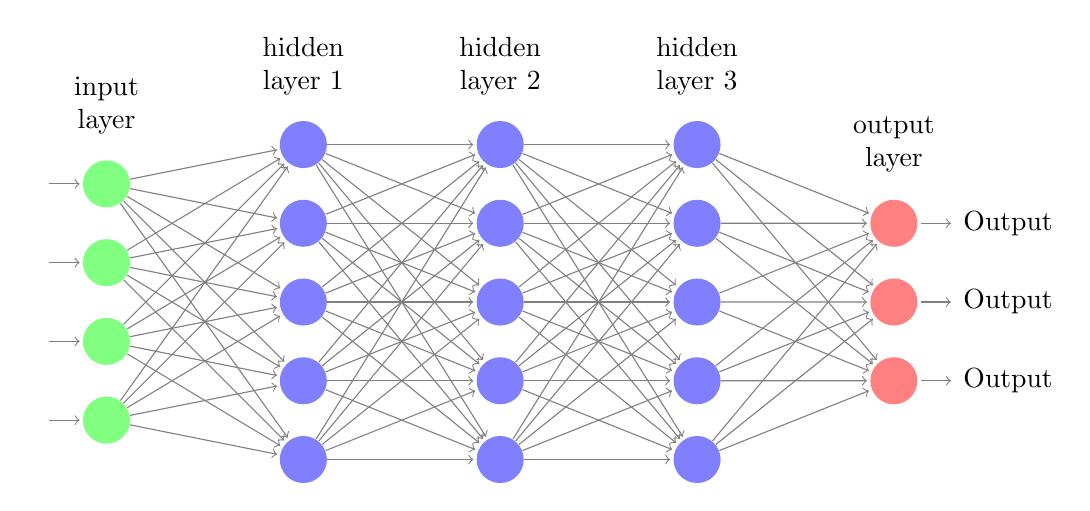
\begin{tikzpicture}[shorten >=1pt,->,draw=black!50, node distance=\layersep]
  \tikzstyle{every pin edge}=[<-,shorten <=1pt]
  \tikzstyle{neuron}=[circle,fill=black!25,minimum size=17pt,inner sep=0pt]
  \tikzstyle{input neuron}=[neuron, fill=green!50];
  \tikzstyle{output neuron}=[neuron, fill=red!50];
  \tikzstyle{hidden neuron}=[neuron, fill=blue!50];
  \tikzstyle{annot} = [text width=4em, text centered]

  % Draw the input layer nodes
  \foreach \name / \y in {1,...,4}
  % This is the same as writing \foreach \name / \y in {1/1,2/2,3/3,4/4}
  \node[input neuron, pin=left:] (I-\name) at (0,-\y) {};

  \node[annot, above of=I-1, node distance=1cm] (il) {input layer};

  % Draw the hidden layer nodes
  \foreach \name / \y in {1,...,5} \path[yshift=0.5cm] node[hidden
  neuron] (H1-\name) at (\layersep,-\y cm) {};

  \node[annot, above of=H1-1, node distance=1cm] (h1l) {hidden layer 1};
  
  \foreach \name / \y in {1,...,5} \path[yshift=0.5cm] node[hidden
  neuron] (H2-\name) at (2*\layersep,-\y cm) {};

  \node[annot, above of=H2-1, node distance=1cm] (h2l) {hidden layer 2};

  \foreach \name / \y in {1,...,5} \path[yshift=0.5cm] node[hidden
  neuron] (H3-\name) at (3*\layersep,-\y cm) {};

  \node[annot, above of=H3-1, node distance=1cm] (h3l) {hidden layer 3};

  % Draw the output layer node
  \foreach \name / \y in {1,...,3} \path[yshift=-0.5cm] node[output
  neuron, pin={[pin edge={->}]right:Output}] (O-\name) at
  (4*\layersep,-\y cm) {};

  \node[annot, above of=O-1, node distance=1cm] (ol) {output layer};

  % Connect nodes
  \foreach \source in {1,...,4}
  \foreach \dest in {1,...,5}
  \path (I-\source) edge (H1-\dest);

  \foreach \source in {1,...,5}
  \foreach \dest in {1,...,5}
  \path (H1-\source) edge (H2-\dest);

  \foreach \source in {1,...,5}
  \foreach \dest in {1,...,5}
  \path (H2-\source) edge (H3-\dest);

  \foreach \source in {1,...,5}
  \foreach \dest in {1,...,3}
  \path (H3-\source) edge (O-\dest);
\end{tikzpicture}
